\documentclass[wcp]{jmlr}
\usepackage{booktabs}
\providecommand{\doi}[1]{\href{https://doi.org/#1}{doi:~\nolinkurl{#1}}}
\hypersetup{pageanchor=false}
\pagenumbering{gobble}
\makeatletter\let\Ginclude@graphics\@org@Ginclude@graphics\makeatother
\jmlryear{2026}
\jmlrworkshop{ACML 2026}
\title[Prediction and Discovery in LipidAL]{Prediction, Discovery, and Explanation in Protein--Lipid Active Learning under Leakage-Controlled Evaluation}
\author{}
\editors{Andy Song, Bo Han and Sarah Erfani}
\begin{document}
\makeatletter\let\@jmlrpages\@empty\makeatother
\maketitle
\begin{abstract}
Acquiring strong binders and predicting binding affinity throughout a chemical
space are distinct objectives. We study this distinction retrospectively using
864 dissociation-affinity and 549 inhibition-affinity protein--lipid pairs from
BioDolphin, together with four exploratory target panels. An initial 5,850-run
representation--kernel--policy benchmark is supplemented by 9,720 campaigns
with cold-sequence and scaffold evaluation, frozen protein language-model
features, and validation-only configuration selection. We implement
prediction-aware Thompson sampling, an equal-rank combination of a joint
posterior affinity draw and conditional predictive variance reduction.
On cold-sequence dissociation data it reduces descriptive mean MAE from
1.541 to 1.406 pK relative to Thompson sampling, but pool top-decile recall
falls from 59.6\% to 23.3\%. The result is a changed trade-off, not joint
superiority. A further 1,296 campaigns evaluate small-corpus lipid
self-supervision and initial-label-only feature adapters; improvements are
inconsistent. Individual-bit nonlinear explanations, background sensitivity,
fingerprint-collision audits, and illustrative contacts in two experimental
complexes extend an earlier temporal SHAP analysis. Six-seed corrected tests
are underpowered and establish no superiority. The study provides auditable
methods and an interactive dashboard, while retaining limitations from assay
heterogeneity, retrospective design, and limited independent biological data.
\end{abstract}
\begin{keywords}
active learning; protein--lipid affinity; Gaussian processes; Thompson sampling;
protein language models; explainability
\end{keywords}

\section{Introduction}
Protein--lipid affinity prediction combines limited measured data, heterogeneous
assays, and chemically diverse ligands. Active learning (AL) can make efficient
use of sequential measurements, but efficiency depends on the objective.
Selecting high-affinity pairs may enrich a measured collection while leaving
poorly covered regions that dominate prediction error. Random-pair evaluation
can further obscure generalization when related proteins and chemistries occur
on both sides of a split.

We adapt the explainable ligand-affinity framework of
\citet{srivastava2026} to protein--lipid pairs. Our original random-pair grid
found different configurations optimal for prediction and discovery. Here we
turn that observation into an explicit dual-purpose selection rule and test
it under harder splits. We do not claim that variance reduction, Thompson
sampling, or their combination is a new theoretical principle. The contribution
is a reproducible domain-specific implementation, matched evaluation, and
careful accounting of where apparent improvements disappear.

The extended study contributes: (i) cold-sequence and scaffold evaluations
with inner-validation model selection; (ii) frozen ESM-2 protein features
crossed with five lipid encodings; (iii) prediction-aware Thompson and a pure
variance-reduction ablation; (iv) leakage-controlled lipid adaptation; and
(v) collision-aware and nonlinear explanation diagnostics, including selected
experimental contacts. The previous 5,850 campaigns remain a separate,
descriptive discovery study. The new 11,016 unique campaigns do not turn that
earlier post-hoc selection into independent validation.

\section{Related Work and Scope}
The ligand-affinity framework compares encodings, GP kernels, and scheduled
exploration and exploitation, with explanations of acquired-model predictions
\citep{srivastava2026}. Gaussian processes provide joint uncertainty
\citep{rasmussen2006}; Thompson sampling queries a correlated posterior
function realization \citep{russo2018}. Predictive variance reduction is a
long-established AL criterion \citep{cohn1996}, and multiobjective batch
selection has substantial prior art \citep{gupta2018}. Accordingly, our
selector is an empirical synthesis requiring comparison, not a novelty claim
based only on a new name.

Frozen molecular encoders, including ChemBERTa and MoLFormer
\citep{chemberta,ross2022}, and protein encoders such as ESM-2
\citep{esm}, can improve representation without fitting every encoder on
scarce affinity labels. They do not guarantee task-specific gains. We compare
two ESM-2 sizes, not two independent architecture families. Domain continued
pretraining and feature adapters are assessed separately from the frozen grid.

SHAP decomposes predictions relative to a background game
\citep{lundberg2017}. An ECFP position can represent multiple hashed
environments \citep{rogers2010}; highlighting one occurrence is not an
identification of a binding site. We distinguish numerical fidelity,
stability, geometric contact evidence, and mechanistic validation.

\section{Data and Evaluation Protocols}
\subsection{Published measurements and endpoint scope}
BioDolphin is a broad lipid--protein interaction resource
\citep{yang2024}; only its curated quantitative affinity-bearing subset is
used. Deduplication is by protein sequence and lipid SMILES, with curated
median consensus labels and censored annotations excluded. Affinity is
expressed as $pK=-\log_{10}(K/\mathrm M)$; larger values indicate stronger
binding. $K_d$ and $K_i$ are kept separate. Imported assay annotations can
originate in other affinity resources; we do not claim BioDolphin generated
all measurements. Its lipid definition is broader than membrane phospholipids.

The pooled endpoints contain 864 $K_d$ and 549 $K_i$ pairs. Across the pooled
sets there are 549 lipids and 1,099 distinct protein sequences. TRAAK panels
use the published mean first sequential binding constant from triplicates
\citep{schrecke2021}; replicates and later binding events are not independent
training pairs. Two sequence-defined transthyretin subsets overlap pooled
$K_d$. These panels are not six independent large biological datasets.

\begin{table}[t]
\centering\small
\caption{Distinct evaluation stages. Additional validation labels in the new
stage are charged separately; final acquisition budgets alone are not total
label cost. Tiny target panels appear only in the original exploratory grid.}
\label{tab:stages}
\begin{tabular}{lrrrl}
\toprule
Stage & Pairs & Seeds & Acquired labels & Selection/splits\\
\midrule
Original pooled $K_d$ &864&3&360&Post-hoc / random pair\\
Original pooled $K_i$ &549&3&360&Post-hoc / random pair\\
TRAAK-a / TRAAK-b &16 / 16&3&8&Exploratory random pair\\
TTR-A / TTR-B &11 / 11&3&8&Exploratory random pair\\
New pooled $K_d$ / $K_i$ &864 / 549&6&120&Inner validation / three splits\\
\bottomrule
\end{tabular}
\end{table}

\subsection{Original random-pair grid}
Seeds 7, 19, and 42 define frozen approximately 20\% test partitions. Pooled
campaigns start with 60 labels and acquire ten batches of 30. Small panels
start with two and acquire six more over ten phase slots, including zero-query
slots. The design crosses six panels, five lipid representations, five
kernels, 13 policies, and three seeds, totaling 5,850 campaigns. Its reported
winners were selected post-hoc from test summaries; these results are
descriptive and not independent evidence of superiority. Test labels did not
guide model fitting or within-campaign acquisition.

\subsection{Cold-sequence, scaffold, and random controls}
The new design uses seeds 7, 19, 42, 73, 101, and 137. Approximately 20\% of
whole groups are assigned to outer test, followed by 20\% of the remainder to
inner validation, subject to group sizes. The remaining acquisition pool
starts with 24 labels and receives four batches of 24. Exact row indices and
costs are recorded. Validation labels are never acquired, but are charged
as additional labels. These 120-label campaigns are not budget-matched to
the original 360-label study.

For cold-sequence evaluation, we compute all-pairs global Needleman--Wunsch
alignments with BLOSUM62, gap-open 10 and extension 1. Identity is matched
residues divided by alignment columns. Connected components join proteins
with identity greater than 40\% or the same recorded accession. Transitivity
is retained; whole components are separated. All cold train/test splits have
maximum global identity below 40\%, with no exact sequence or recorded
accession overlap. This operational definition does not establish curated
family separation or exclude similar local domains.

Scaffold splits group nonchiral Bemis--Murcko scaffolds. All acyclic molecules
share one group rather than being separated by their full SMILES. Random-pair
splits provide a matched easier control. For each policy and partition, final
inner-validation MAE selects representation and kernel, with deterministic
lexical tie-breaking. Protein-specific comparisons select lipid/kernel while
holding the protein representation fixed. This is repeated nested holdout
with a single inner split, not full nested $K$-fold cross-validation. Outer
test results never select configurations or candidates.

\subsection{Metrics and inference}
We report test MAE, $R^2$, interval coverage, acquisition-pool top-decile
recall, and label-normalized recall AUC. Recall includes initial and acquired
pairs and is not a test classification score. Changing split regimes changes
the eligible pool and group composition; differences are protocol sensitivity,
not a controlled estimate of leakage alone.

Exploratory paired two-sided sign-flip tests use six seed-level differences,
comparing prediction-aware Thompson with Thompson and uncertainty on MAE and
recall AUC across six endpoint/split settings. Holm correction spans 24 tests.
With six signs the smallest possible two-sided exact $p$ is $2/64=0.03125$;
the smallest attainable Holm-adjusted value in this family is 0.75. The
analysis is therefore underpowered by construction. Overlapping holdouts are
not independent biological replications; absence of significance does not
establish equivalence. Future confirmatory work needs predeclared primary
comparisons and independently justified sample size.

\section{Models and Acquisition}
\subsection{Frozen representations and GP fitting}
Lipid representations are radius-four, 4,096-bit ECFP, 167-bit MACCS,
384-dimensional ChemBERTa-MTR and ChemBERTa-MLM, and 768-dimensional
MoLFormer-XL. Model revisions, feature hashes, and preprocessing are saved.
MoLFormer removes stereochemistry as in its pretraining pipeline; representation
comparisons therefore also reflect preprocessing assumptions. The original
protein representation is a 26-dimensional composition/length/charge feature
vector, not a learned structural encoding.

The new grid adds frozen ESM-2 8M and 35M features of dimensions 320 and 480.
Mean residue pooling excludes special tokens. Five proteins longer than
1,000 residues are encoded in disjoint chunks and residue-weighted pooled;
this avoids truncation but loses cross-chunk context. These encoders are not
trained on the benchmark affinities. ESM-2 was pretrained externally, so
benchmark sequence novelty relative to pretraining is not established.

The pairwise exact GP combines lipid covariance with a protein RBF factor
when proteins vary. Initial-set statistics scale inputs and distances;
only acquired labels determine target normalization. The original grid uses
linear, Tanimoto, RBF, rational quadratic, and Mat\'ern-$3/2$ lipid kernels.
The new matched grid uses linear, RBF, and Mat\'ern-$3/2$, spanning previous
winner families without claiming an exhaustive kernel search. Constant mean,
signal/noise variances, and applicable kernel parameters are fitted using
analytic-gradient L-BFGS-B with warm starts and at most 60 iterations.
New protein geometry is explicitly float64. A failed earlier float32 attempt
is invalidated and excluded, not pooled with completed results.

\subsection{Baselines and prediction-aware Thompson}
The original suite contains uniform random, balanced UCB, five scheduled
exploration and exploitation policies, joint Thompson, greedy mean, pure
uncertainty, expected improvement, probability of improvement, and a fixed
Thompson--diversity heuristic. EI/PI use marginal top-$k$ scores, not joint
batch EI. The new grid retains random, uncertainty, balanced UCB, and joint
Thompson, adding the proposed implementation and pure variance reduction.

Let $C$ be latent posterior covariance and $\tau^2$ fitted observation noise
in output units. A fixed proxy set $V$ contains at most 64 inner-validation
inputs, selected without labels. For a candidate $x$, define
\begin{equation}
g(x)=\frac{1}{|V|}\sum_{v\in V}
\frac{C(v,x)^2}{C(x,x)+\tau^2}.
\label{eq:gain}
\end{equation}
This is the integrated reduction in proxy latent variance for one noisy
observation with fixed GP hyperparameters, not expected reduction in MAE.
Draw one correlated latent posterior function over the candidate pool,
$\widetilde{\boldsymbol f}\sim\mathcal N(\boldsymbol\mu,\boldsymbol C)$.
Prediction-aware Thompson greedily scores unselected candidates by
\begin{equation}
s(x)=(1-\lambda)\operatorname{rank}_{[0,1]}\{\widetilde f(x)\}
+\lambda\operatorname{rank}_{[0,1]}\{g(x)\},\qquad\lambda=0.5.
\end{equation}
Ranks use average ties and are recomputed among remaining candidates. After
each selection, condition the covariance using the noisy-observation Schur
update before computing the next gain. The original function draw is retained
within the batch. Pure variance reduction uses $\lambda=1$; standard Thompson
is separately implemented as the existing baseline. No weight search uses
test outcomes. The selector receives proxy inputs but neither proxy labels
nor outer-test inputs/labels. Covariance conditioning needs no fantasized
labels; hyperparameters remain fixed within the batch.

The main grid is $2\times3\times6\times3\times5\times3\times6=9,720$
campaigns. All policies have the same initial rows, split, and budget within
a partition. Formula checks match direct variance changes to
$3.27\times10^{-15}$ at worst. These checks establish implementation fidelity,
not that variance is calibrated or that the chosen scalarization is optimal.

\section{Lipid-Domain Adaptation}
Label-free continued ChemBERTa MLM training begins from the pinned frozen
checkpoint. Of 2,615 unique raw BioDolphin SMILES, seven fail RDKit validation.
Excluding all benchmark scaffolds, including the acyclic group, and
overlength token sequences leaves 790 molecules. This is a small pilot,
not large-scale LMSD or SwissLipids pretraining. Three fixed epochs use
15\% masking with the standard 80/10/10 masking rule, learning rate
$10^{-5}$, batch size 16, and seed 7. Embeddings are then frozen. Decreasing
training loss is not independent evidence of better affinity representation.

The supervised alternative fits residual bottleneck feature adapters to
ESM-2 35M and ChemBERTa-MLM embeddings using only each partition's 24 initial
labels. Bottleneck width is 32, residual scale 0.1, and final residual weights
start at zero. A small predictive head optimizes standardized affinity MSE
plus a 0.01 residual penalty with AdamW, learning rate 0.001, weight decay
0.01, and 100 fixed epochs. Adapted features are returned in the original
feature units, avoiding a hidden scaling change. Each of 36 adapters is
frozen and reused across policies/kernels before any acquisition. No future
labels or full pooled-label fine-tuning are used. These are feature adapters,
not attention LoRA or supervised transformer-weight updates.

The matched adaptation comparison fixes ESM-2 35M and the MLM lipid family,
varying frozen, self-supervised, and adapter variants across all partitions,
three kernels, and six policies. Its 1,944 entries include 648 frozen
baselines already counted in the main grid, hence 1,296 additional campaigns.
Kernel choice is by inner-validation MAE within each variant/policy.

\section{Results}
\subsection{Original results and budget context}
In the original post-hoc search, ECFP--linear uncertainty gives lowest
descriptive pooled MAE: $0.641\pm0.041$ for $K_d$ and $0.429\pm0.044$ for
$K_i$. The lowest-MAE $K_d$ Thompson configuration, MTR--Mat\'ern, has MAE
$0.705\pm0.046$ and recall 0.967. Balanced UCB with MLM--linear has the
highest $K_d$ recall AUC, 0.783, while greedy and exploit-heavy MTR--linear
tie at 0.864 on $K_i$. These winners optimize different objectives. The
$K_i$ budget already covers about 82\% of its acquisition pool; final recall
alone can look favorable even without exceptional early discovery.

All tiny panels retain negative mean $R^2$ even for their lowest-MAE selected
configurations. No reliable target-level prediction claim follows from
11--16 pairs. Full original tables and all historical figures remain in the
supplement; their selections are not mixed with the validation-selected stage.

\begin{figure}[t]
\centering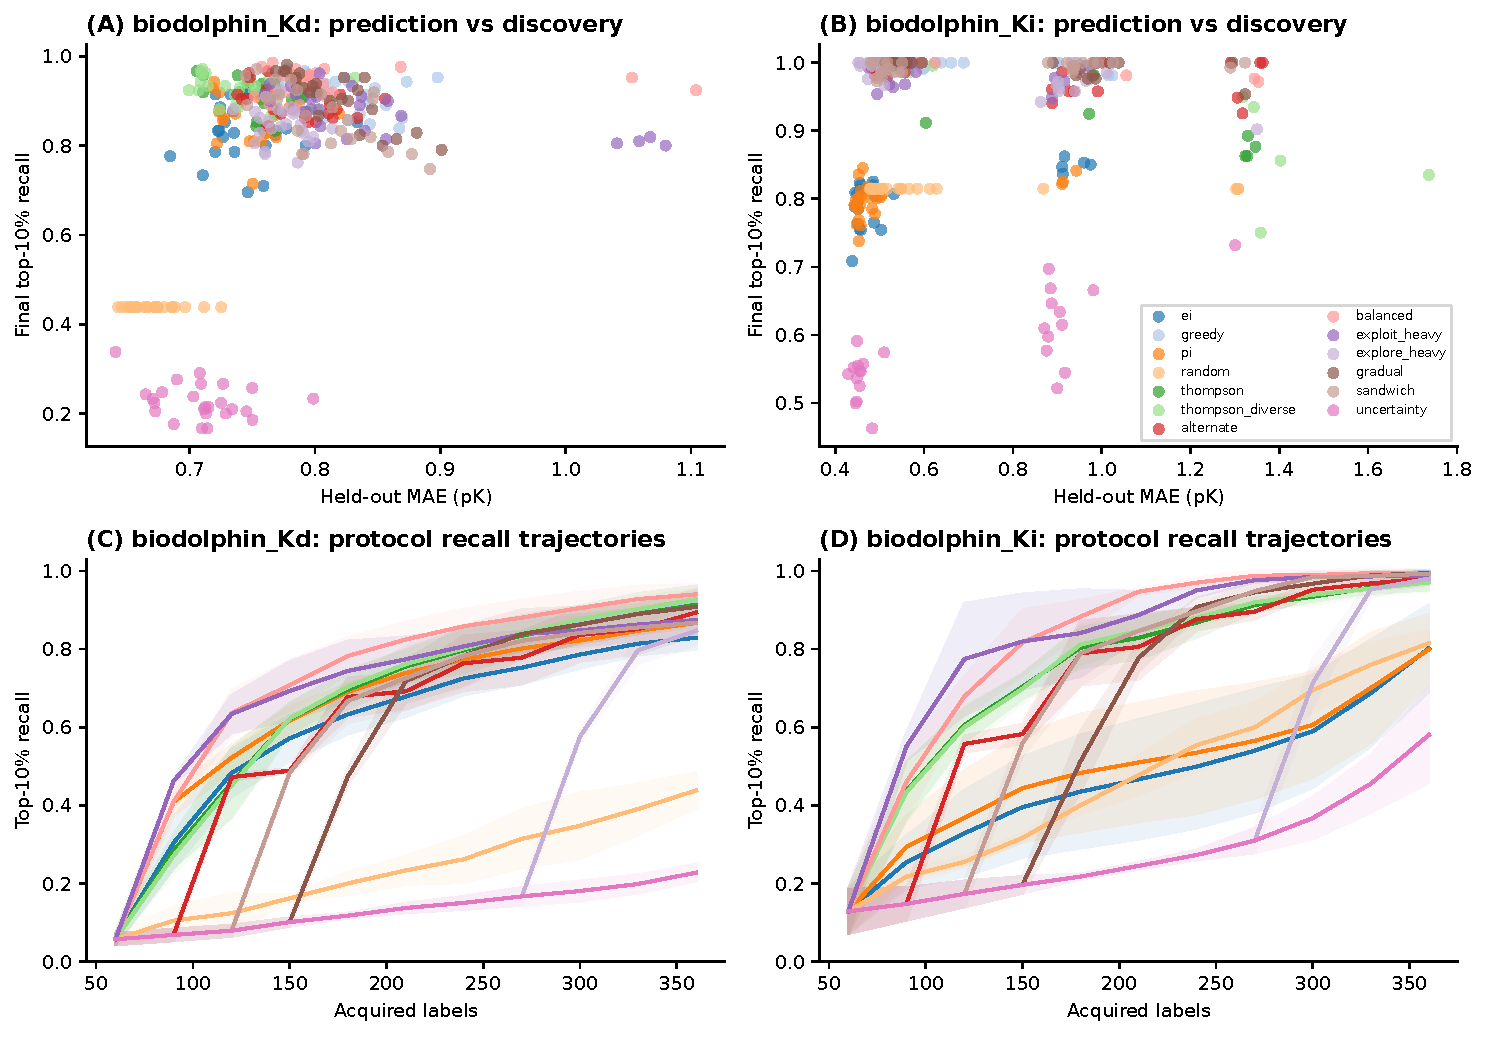
\includegraphics[width=\linewidth]{figures/fig1_performance.pdf}
\caption{Original descriptive four-panel benchmark: prediction and discovery
rank configurations differently. Pooled acquisition budgets are 360 labels;
these curves are not budget-matched to the new 120-label study. Means across
three seeds and post-hoc choices are exploratory.}
\label{fig:original}
\end{figure}

\subsection{Leakage-controlled evaluation exposes a harder task}
Table~\ref{tab:new} and Figure~\ref{fig:policy} show validation-selected
six-seed outcomes. For prediction-aware Thompson, random-pair MAE is 0.933
on $K_d$ and 0.702 on $K_i$, increasing to 1.406 and 1.428 on cold sequence,
and 1.277 and 1.336 on scaffold splits. Random acquisition remains competitive:
cold-sequence random MAE is 1.482 on $K_d$ and 1.333 on $K_i$. Harder splits
are essential to interpret the favorable original random-pair results.

\begin{table}[t]
\centering\small
\caption{Validation-selected six-seed means at 120 acquired labels plus
validation cost. TS: Thompson; PA: prediction-aware Thompson. Recall is
acquisition-pool top-decile recovery. No corrected superiority is established.}
\label{tab:new}
\begin{tabular}{llrrrr}
\toprule
Endpoint & Split & TS MAE & PA MAE & TS recall & PA recall\\
\midrule
$K_d$ & Random &1.017&0.933&.513&.311\\
$K_d$ & Cold sequence &1.541&1.406&.596&.233\\
$K_d$ & Scaffold &1.305&1.277&.510&.264\\
$K_i$ & Random &0.895&0.702&.643&.333\\
$K_i$ & Cold sequence &1.419&1.428&.664&.319\\
$K_i$ & Scaffold &1.469&1.336&.879&.340\\
\bottomrule
\end{tabular}
\end{table}

Prediction-aware Thompson improves descriptive MAE over Thompson in five
of six settings, but reduces recall in all six. On cold $K_i$, even MAE is
slightly worse. Balanced UCB often has higher recall, whereas pure variance
reduction frequently sacrifices discovery without achieving lowest MAE.
Thus adding variance reduction does not resolve the trade-off; it provides
an explicit operating point. No calibrated clinical, experimental-cost, or
economic utility has been specified to justify this operating point as best.

\begin{figure}[t]
\centering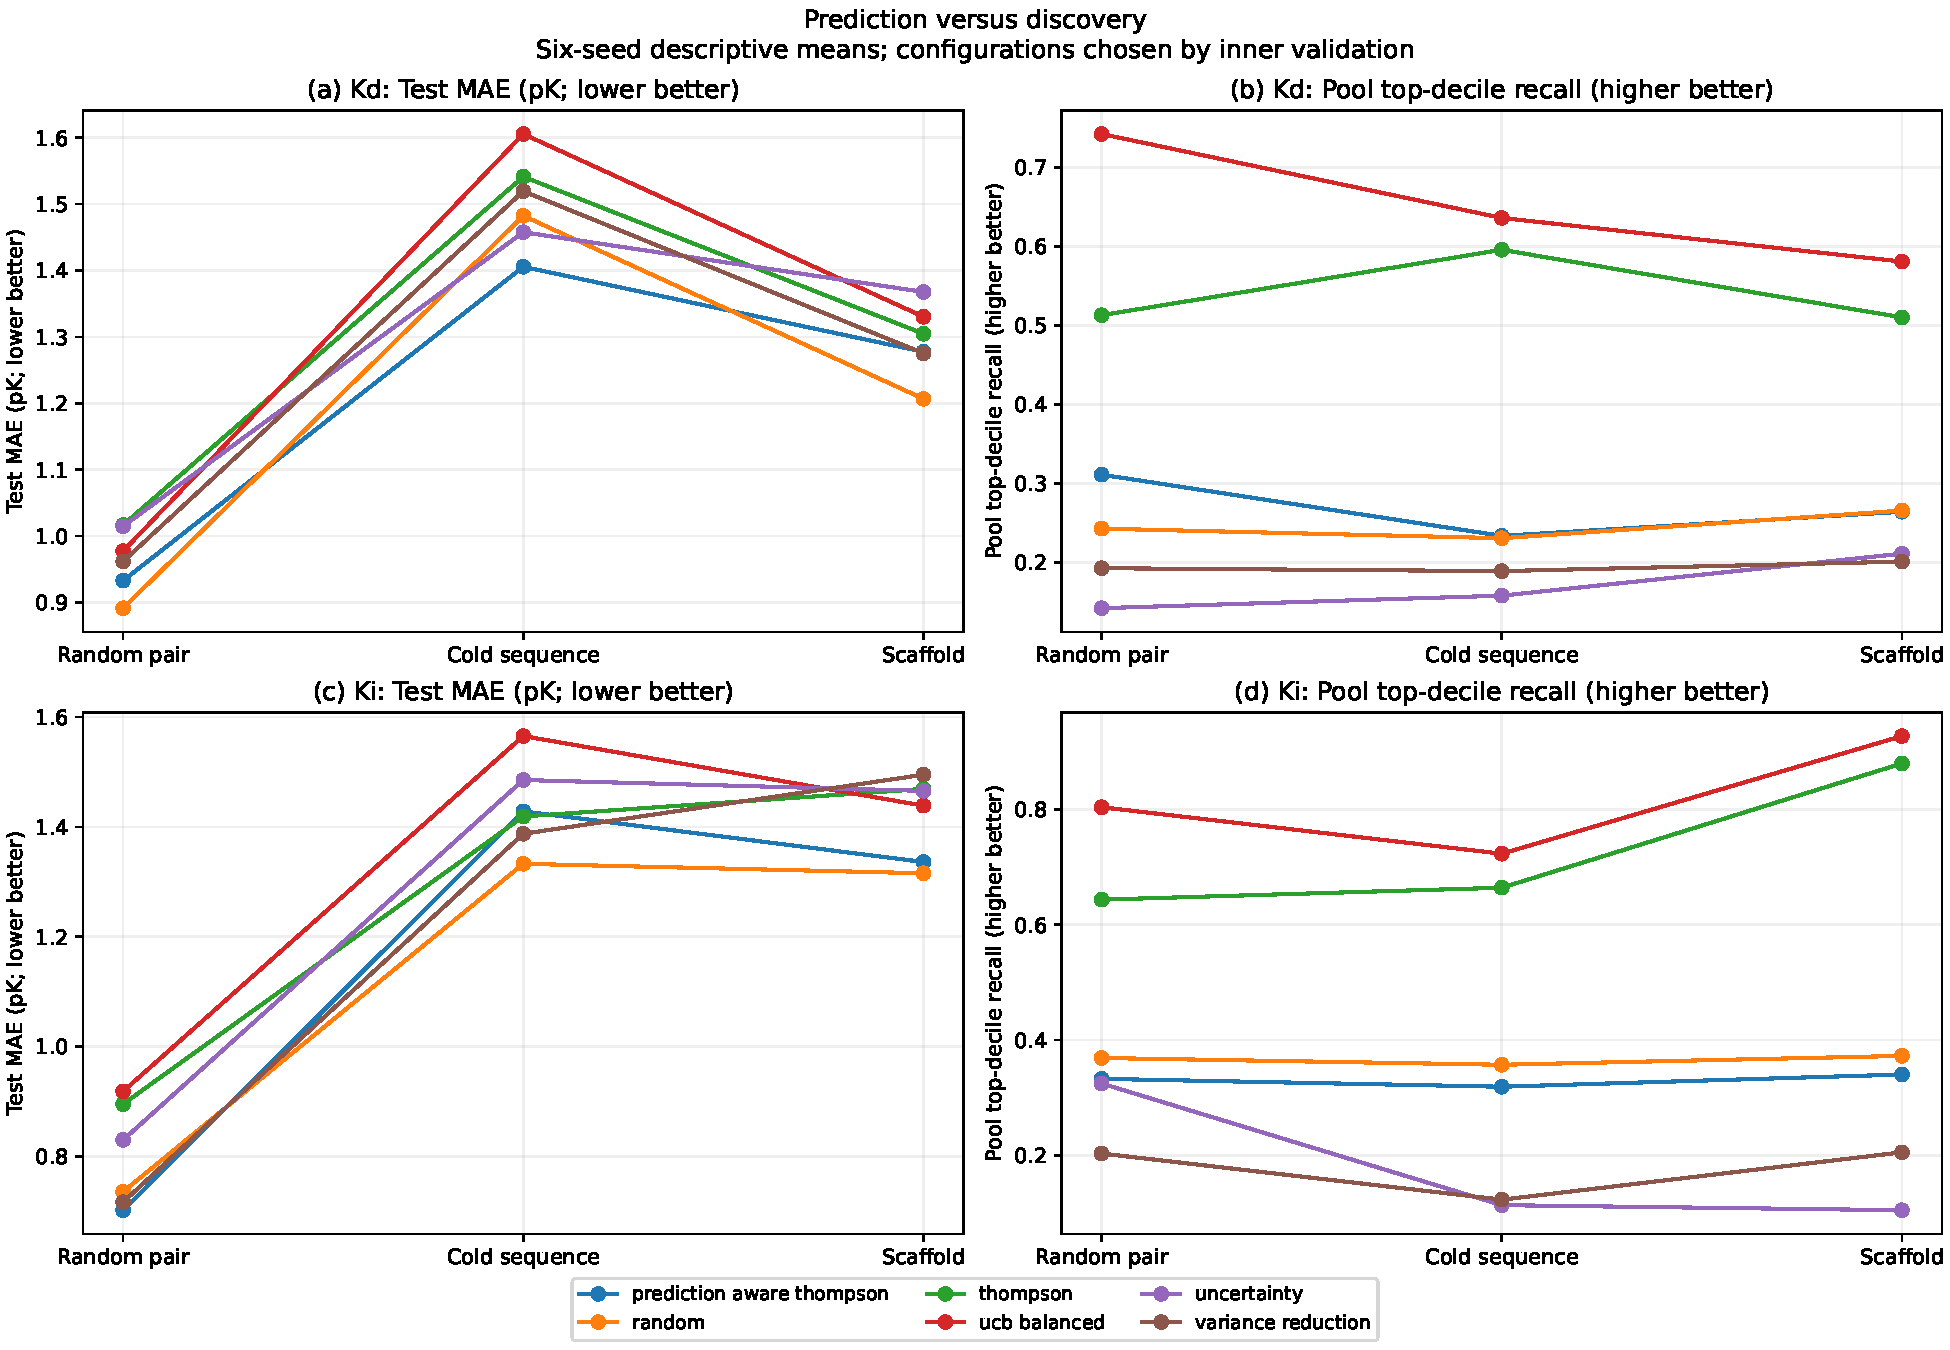
\includegraphics[width=\linewidth]{figures/policy_panels.pdf}
\caption{New six-policy study in four panels: outer-test MAE and pool recall
for $K_d$ and $K_i$. Each point is a six-seed mean after inner-validation
configuration selection. Lines connect split regimes for readability, not
time; no uncertainty bands or significance claims are implied. Raw seed
values and SD summaries accompany the paper.}
\label{fig:policy}
\end{figure}

\subsection{Protein and lipid representation gains are mixed}
Figure~\ref{fig:protein} holds prediction-aware Thompson fixed and selects
lipid/kernel separately within each protein representation. Cold $K_i$ MAE
is 1.446 for composition, 1.411 for ESM-2 8M, and 1.368 for ESM-2 35M.
Cold $K_d$ values are 1.471, 1.482, and 1.451. On scaffold $K_d$, the
8M encoder is descriptively best among these three (1.223 versus 1.295
composition and 1.259 for 35M). Model size therefore does not produce a
monotonic improvement. These conditional comparisons differ from allowing
inner validation to select the protein representation too.

\begin{figure}[t]
\centering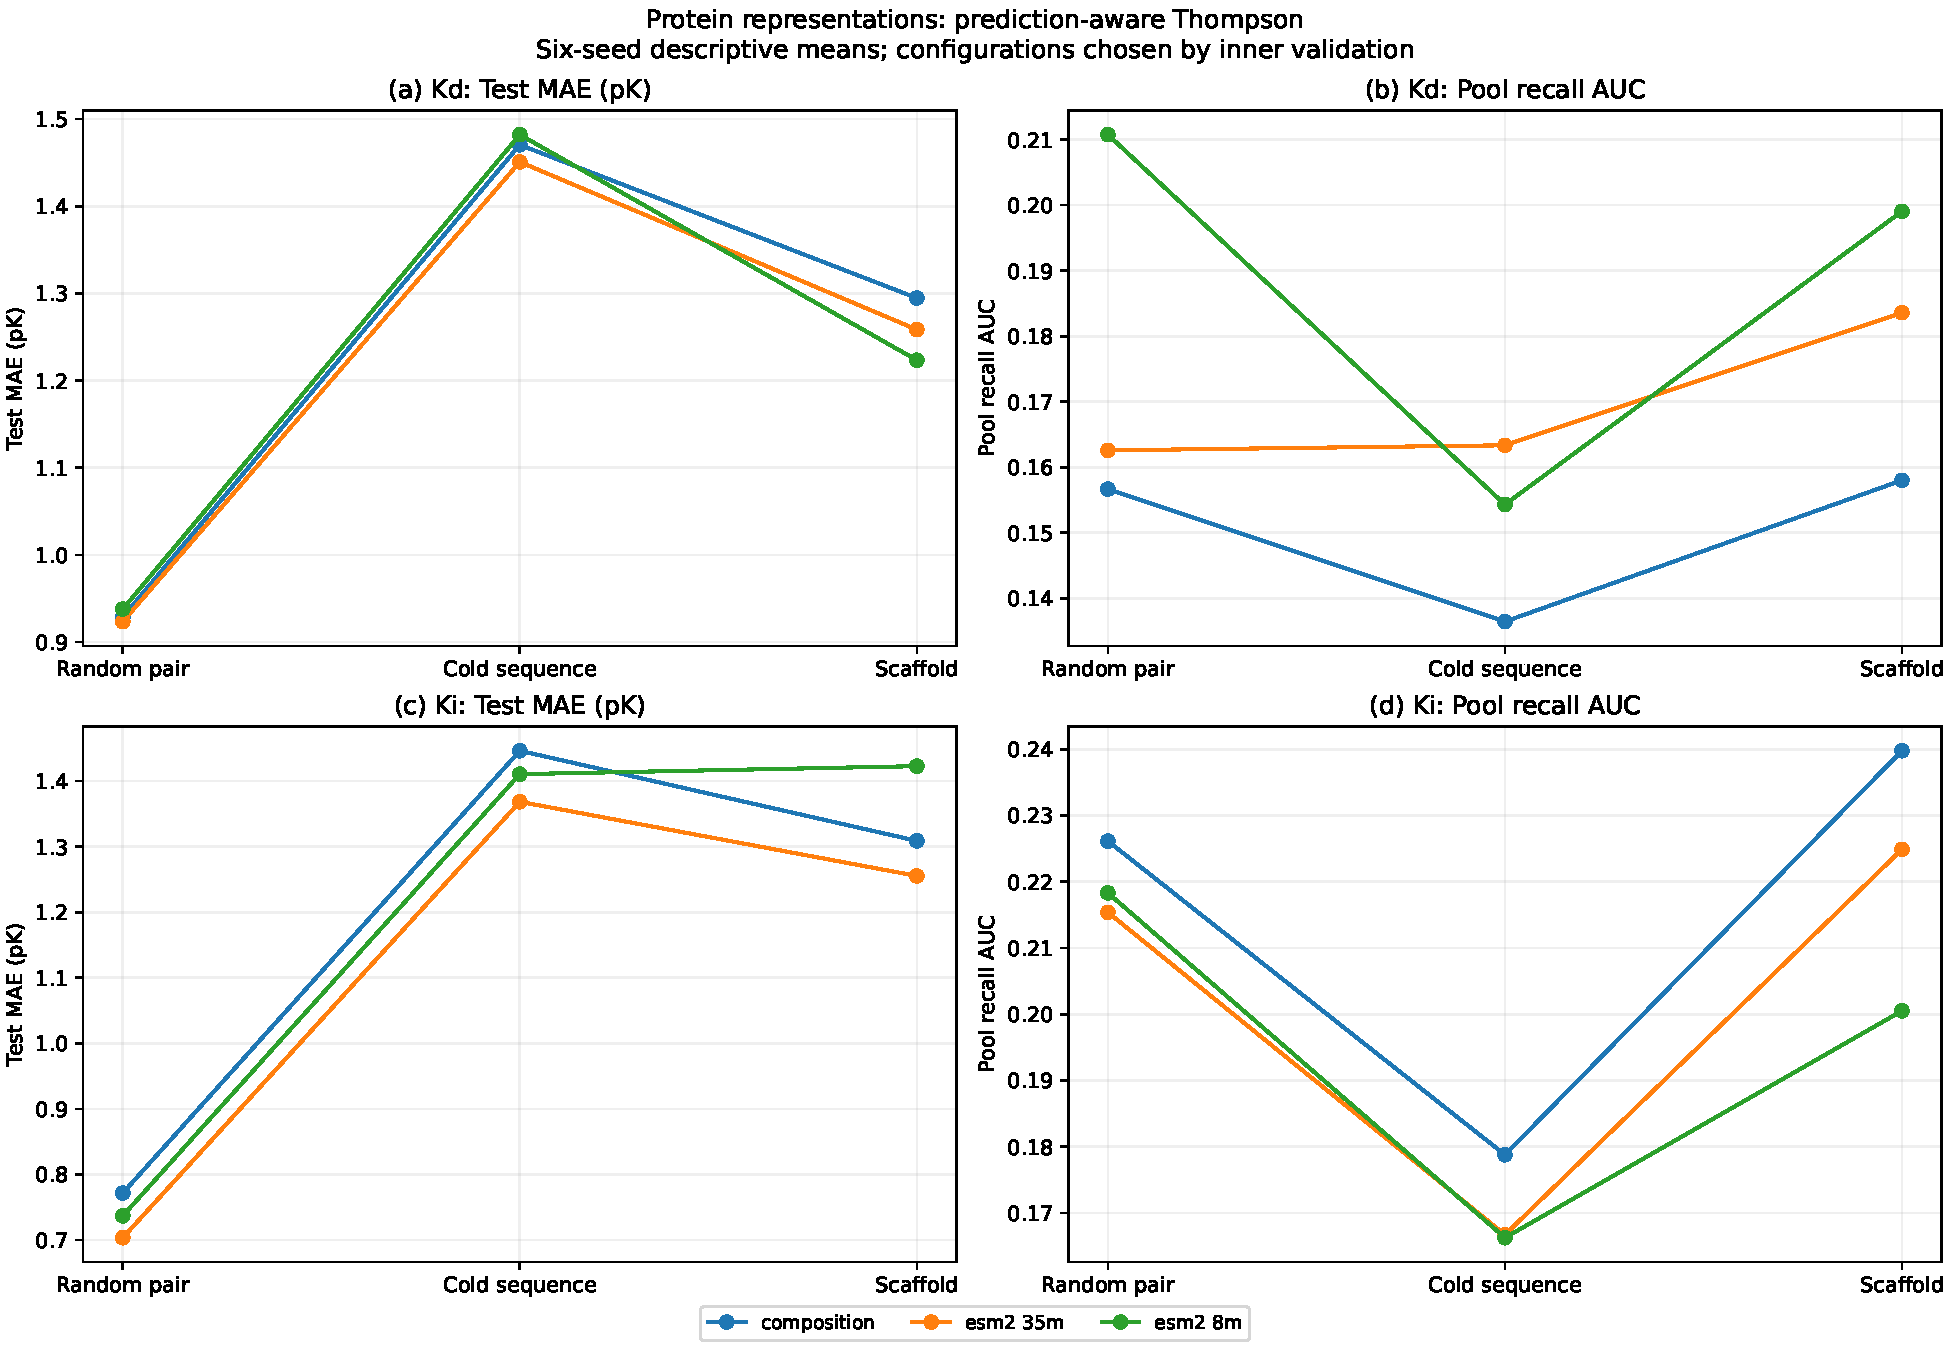
\includegraphics[width=\linewidth]{figures/protein_panels.pdf}
\caption{Four-panel protein comparison for prediction-aware Thompson. Lipid
representation and kernel are chosen by inner validation within each protein
group. The two ESM-2 sizes are one architecture family; differences include
checkpoint pretraining and dimension, not only a controlled capacity change.}
\label{fig:protein}
\end{figure}

The adaptation study also has mixed outcomes (Figure~\ref{fig:adaptation}).
For prediction-aware Thompson on cold $K_d$, frozen / adapter / SSL MAE is
1.431 / 1.416 / 1.520. Cold $K_i$ gives 1.567 / 1.692 / 1.562. Scaffold
$K_d$ improves descriptively to 1.252 with adapters and 1.219 with SSL,
from 1.295 frozen. These comparisons fix the MLM lipid family and should
not be confused with the full five-representation selected results.
There is no separate confirmatory adaptation significance claim.

\begin{figure}[t]
\centering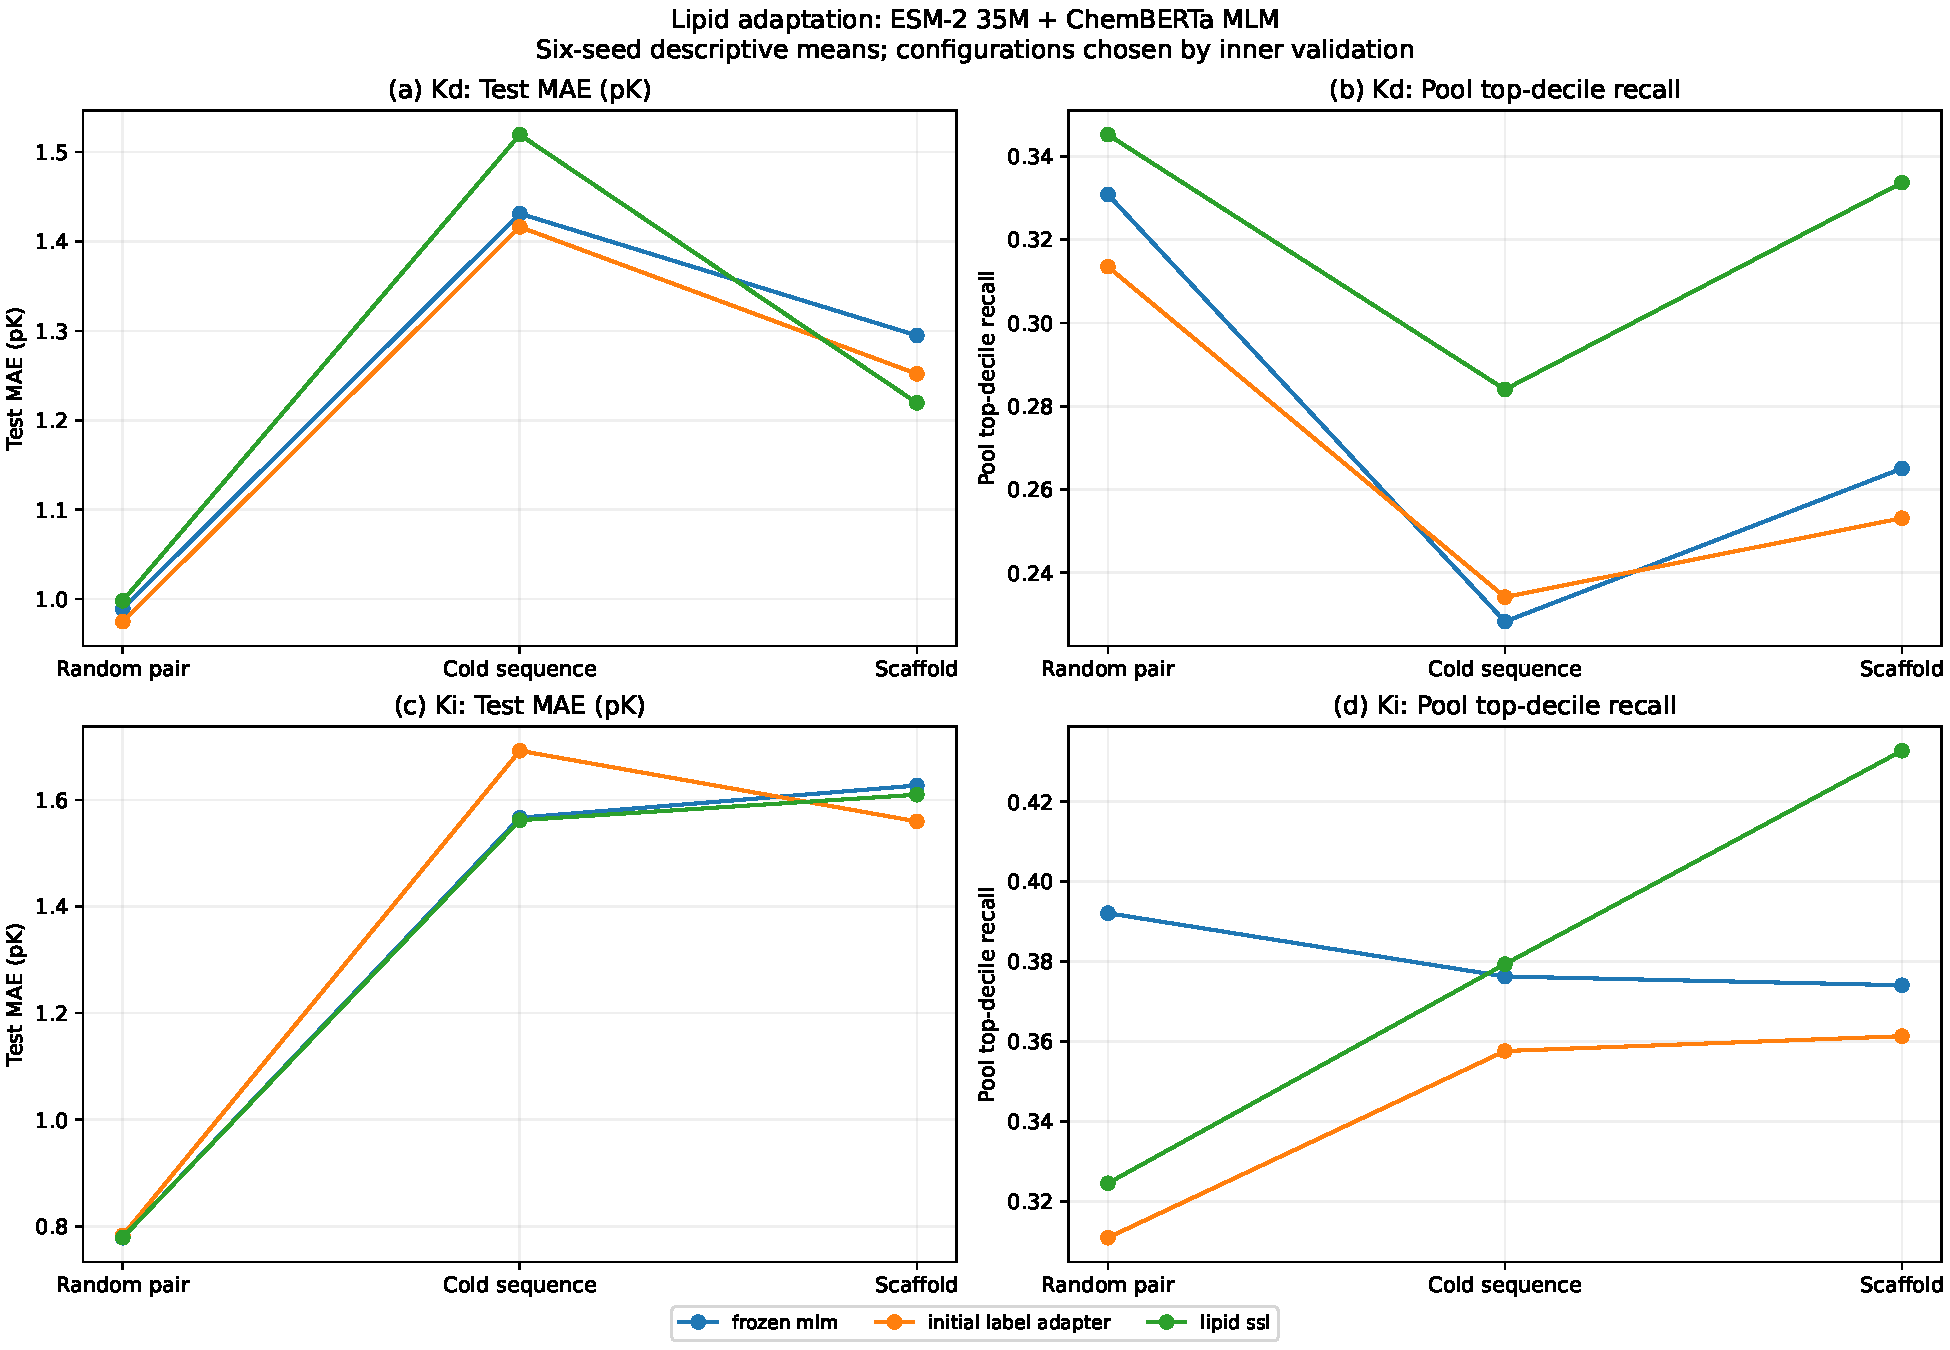
\includegraphics[width=\linewidth]{figures/adaptation_panels.pdf}
\caption{Four-panel matched adaptation comparison using ESM-2 35M,
ChemBERTa-MLM family features, and prediction-aware Thompson. Only kernels
are selected by inner validation. Initial-label adapters and a 790-molecule
SSL pilot do not yield consistent gains; 648 frozen baselines are reused,
not counted as additional unique experiments.}
\label{fig:adaptation}
\end{figure}

\section{Explanation Analysis and Structural Checks}
\subsection{Grouped and temporal explanations}
Historical grouped SHAP reports cover 54 selected final models. The temporal
analysis covers 36 ECFP--linear campaigns, 396 snapshots, and 14,754
query-model explanations with the query protein fixed. Affine conditional
predictions admit exact individual-bit contributions; independent
KernelExplainer comparisons agree below $10^{-10}$ pK. This establishes
computational fidelity for the specified background game, not uniqueness of
the explanation or causal importance.

Backgrounds and unqueried populations can change across cycles. Importance
trajectories therefore combine changes in the model and explained population;
they are not pure longitudinal biological signals. Affinity-prioritized
fragment display uses measured labels retrospectively, including held-out
rows. Those labels do not enter SHAP, querying, or fitting but make the
illustrations unsuitable as independent validation.

\begin{figure}[t]
\centering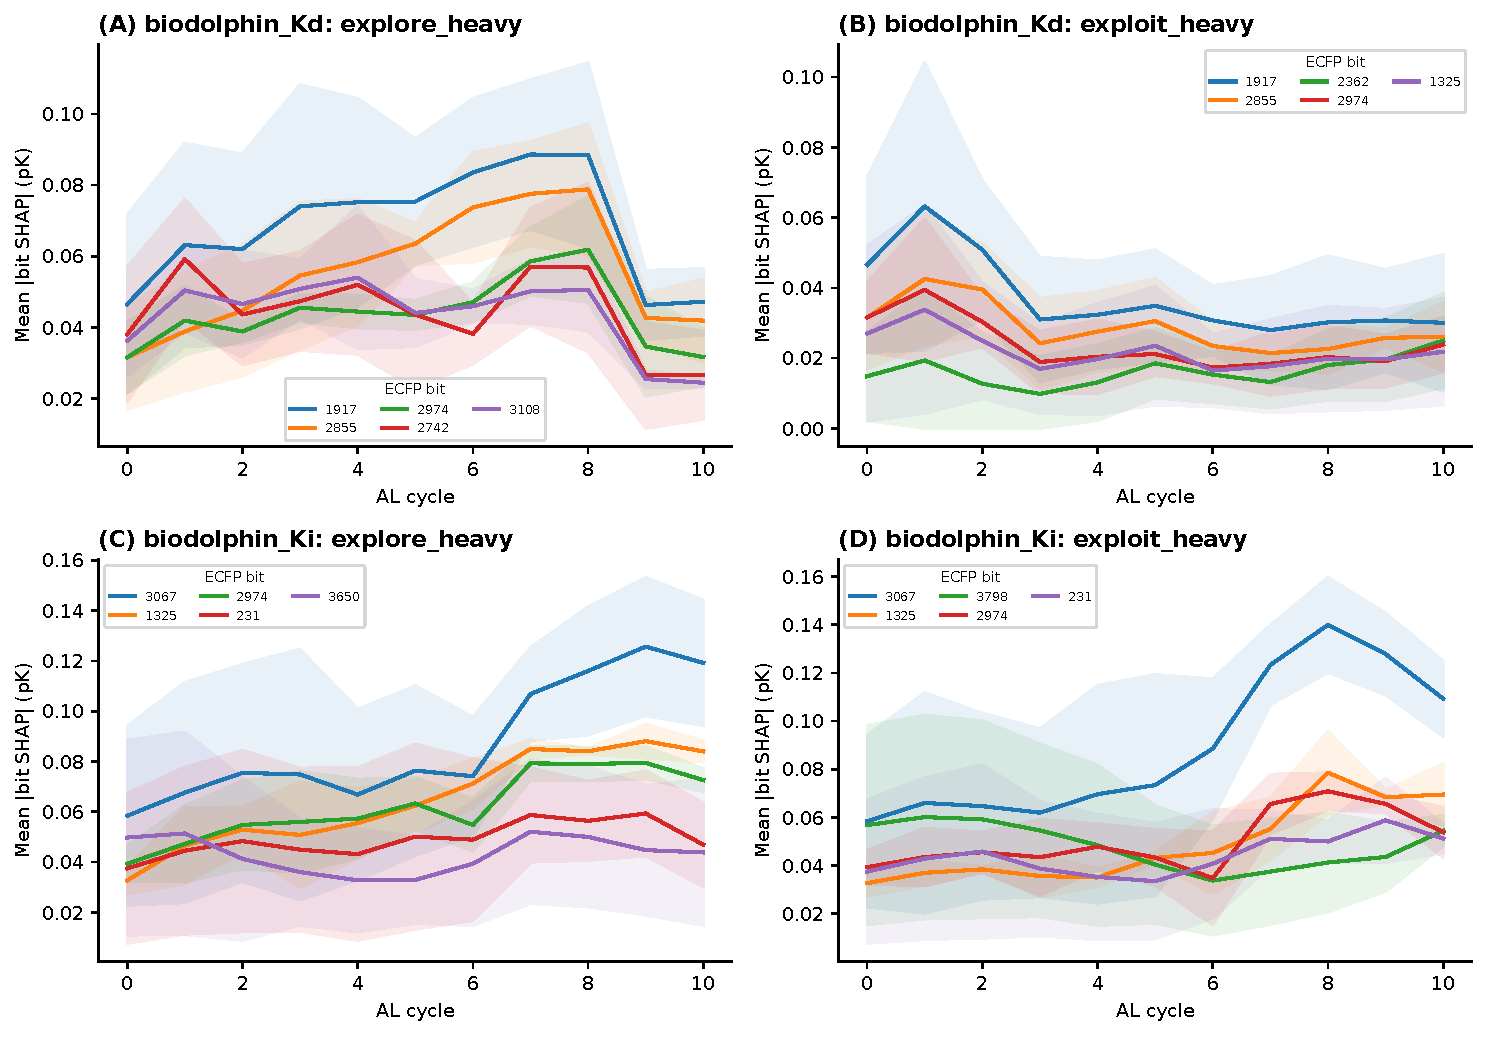
\includegraphics[width=\linewidth]{figures/fig3_temporal.pdf}
\caption{Four historical ECFP--linear temporal panels. The five bits with
largest final seed-averaged importance are shown; bands are seed SD.
Explore-heavy and exploit-heavy schedules are contrasted. Changing
background/query populations prevents a causal interpretation of trajectory
changes. These are the original 360-label campaigns.}
\label{fig:temporal}
\end{figure}

\subsection{Hash collisions and nonlinear background sensitivity}
Across the 549 lipids, 3,539 of 3,980 observed ECFP positions contain more
than one distinct unfolded Morgan identifier. Folding sets are verified
against the actual fingerprint. Even a 32-bit unfolded identifier is not
proof of unique chemistry, and fragment strings have contextual limitations.
High/low-affinity collision comparisons use all labels retrospectively and
are not independently validated structure--activity relationships.

We additionally estimate individual-bit permutation Shapley values for four
prespecified historical nonlinear models: $K_d$/$K_i$ crossed with RBF and
Mat\'ern, ECFP, Thompson, seed 7. Two fixed test queries per model, three
eight-pair acquired-training backgrounds, and two repeats yield 48
explanations. Each estimate uses eight antithetic permutations; protein
features are fixed. Dummy bits are exactly zero. Coalition predictions are
evaluated from exact GP sufficient statistics; attribution estimation itself
is approximate. Additivity does not prove convergence.

Mean top-ten Jaccard across backgrounds is 0.698 for RBF and 0.721 for
Mat\'ern, versus 0.970 and 1.000 for same-background repeats. In this small
diagnostic set, background choice affects ranking more than repeat sampling.
The few models and queries do not support a broad robustness guarantee.

\subsection{Experimental contact illustrations}
We match four affinity-prioritized historical fragment examples to experimental
complexes 4OAS and 6CDJ using recorded BioDolphin source identifiers, chains,
residues, and ligand CCD codes. There are only two distinct complexes, not
four independent confirmations. Full heavy-atom graph matches are used,
with 24 and 16 symmetry mappings respectively; no absent atoms are invented.
Mapping ignores chirality. A contact is a heavy-atom distance at most
4~\AA\ to the recorded protein chain in the first PDB model, without
biological-assembly expansion.

All atoms in these small highlighted fragments contact the protein under
all enumerated mappings. The 4OAS examples contact HIS96, LYS94, and VAL93;
6CDJ examples contact GLY48 or GLY48/49. About 54\% and 51\% of all ligand
atoms, respectively, also satisfy the cutoff. Selected-contact agreement is
therefore illustrative, not proof that high SHAP uniquely localizes a binding
site. No docking, binding-energy decomposition, residue attribution,
prospective mutagenesis, or global contact-map validation is claimed.

\begin{figure}[t]
\centering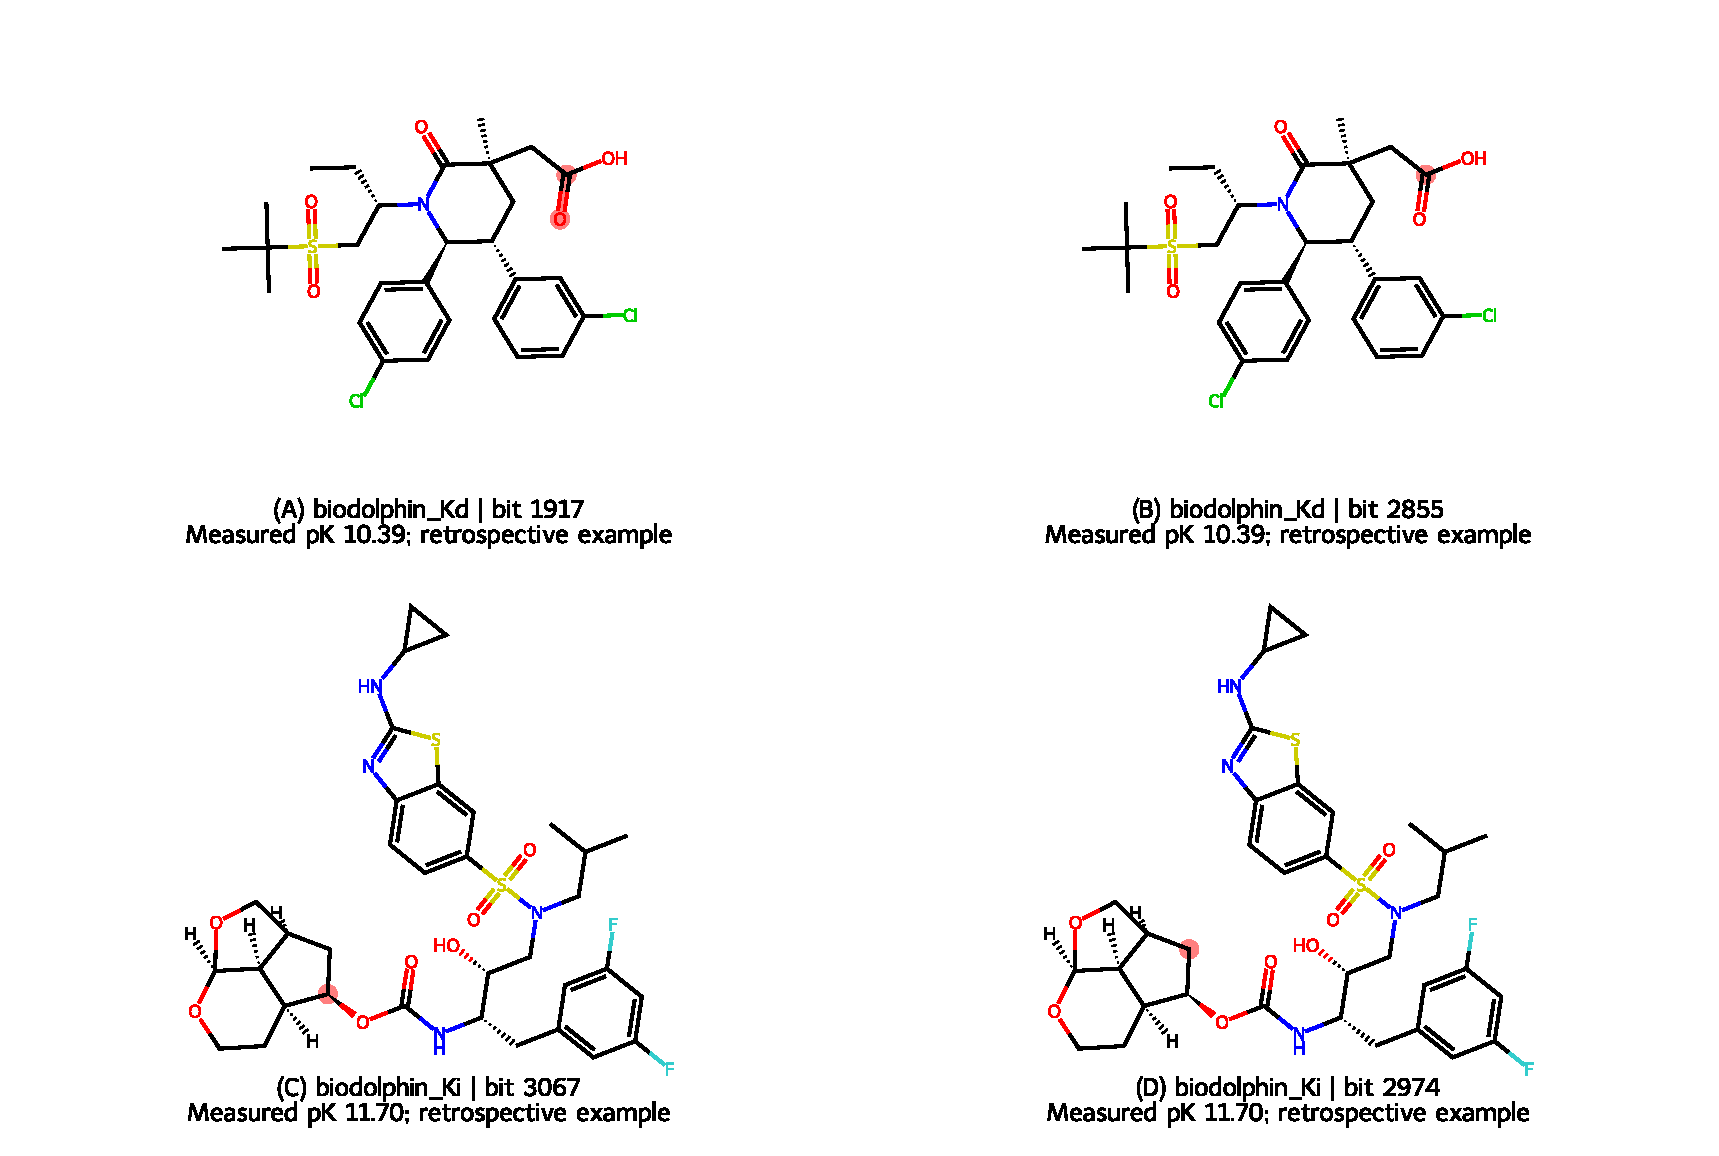
\includegraphics[width=\linewidth]{figures/fig5_fragments.pdf}
\caption{Four historical affinity-prioritized fragment panels, subsequently
checked against two experimental complexes. Highlighting shows a recorded
ECFP environment, not a unique motif or a newly discovered binding site.
The same molecule may appear for different bits. Geometric contact checks
are reported separately and do not make these selected examples causal.}
\label{fig:fragments}
\end{figure}

\begin{figure}[t]
\centering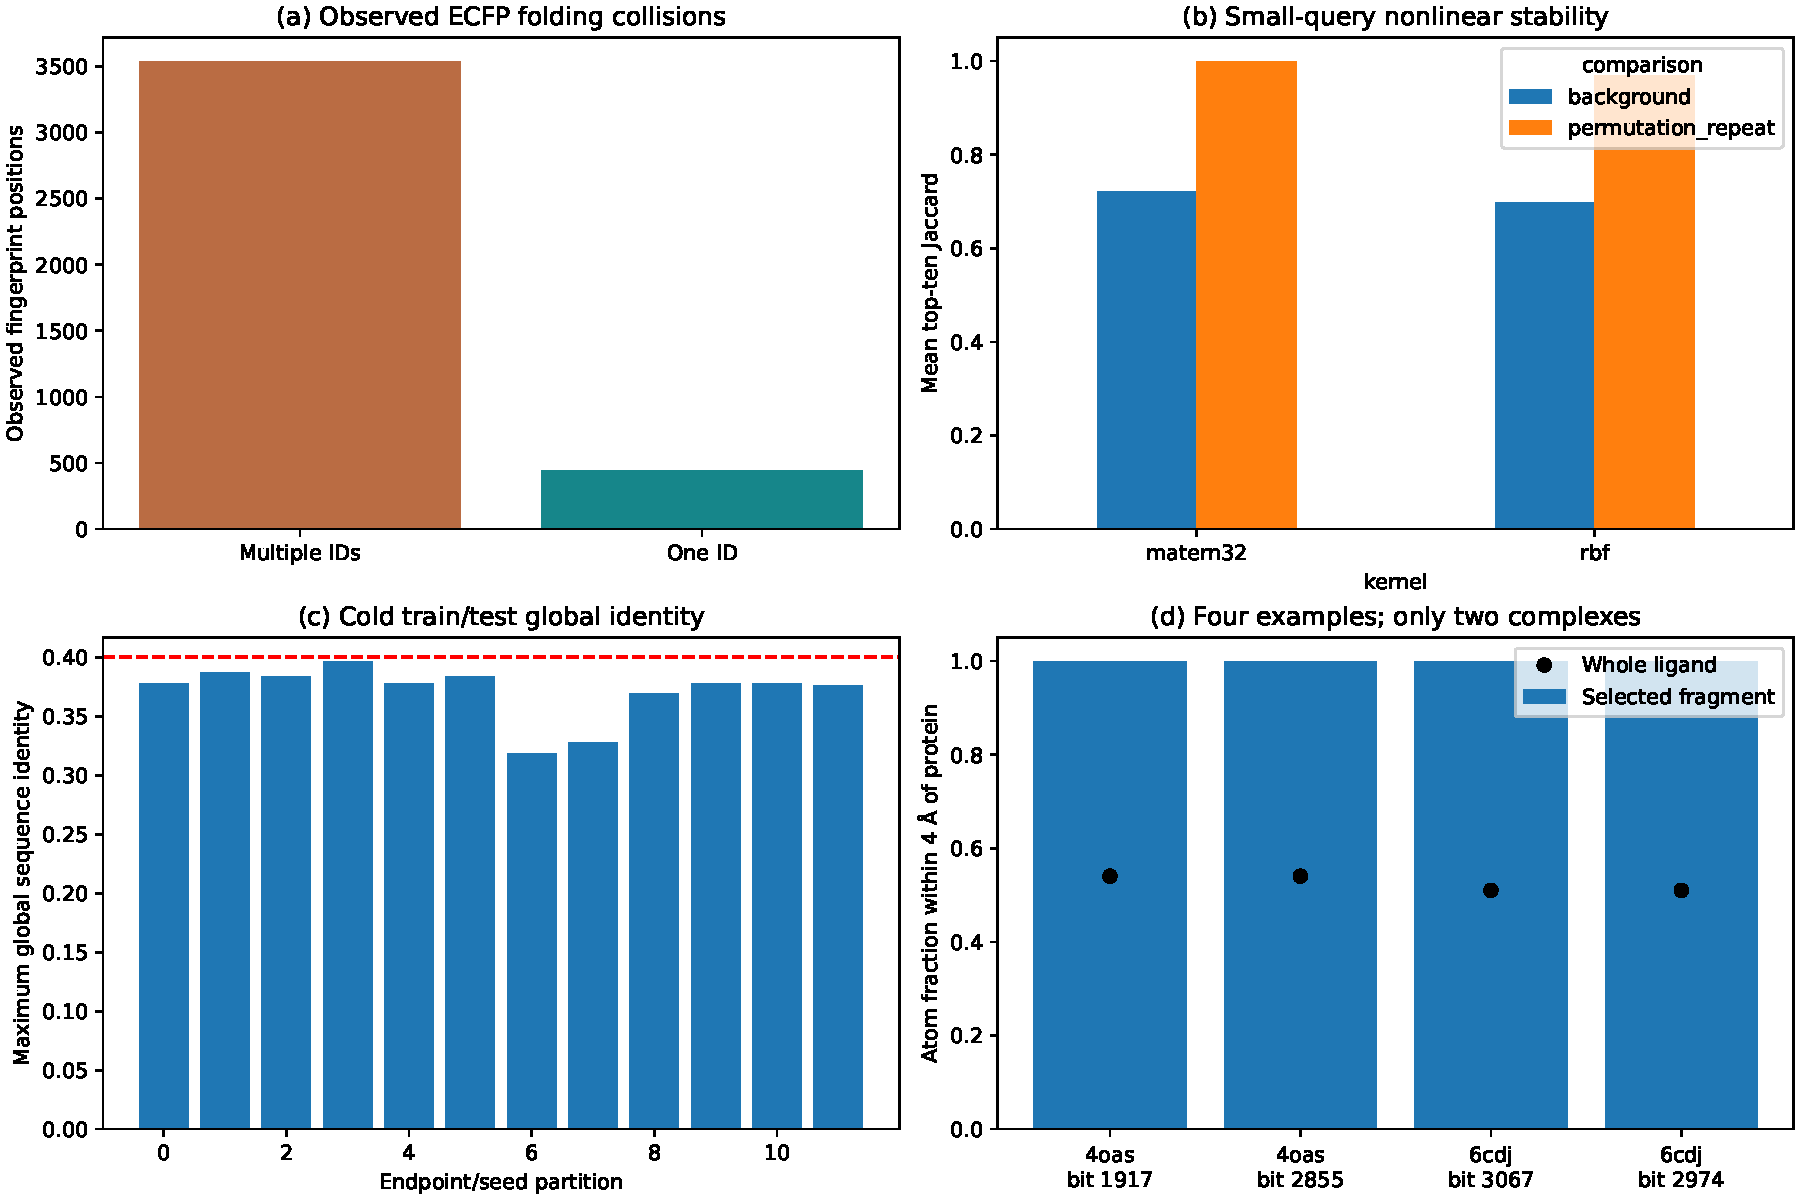
\includegraphics[width=\linewidth]{figures/explanation_checks.pdf}
\caption{Four diagnostics: (a) multiple unfolded identifiers per observed
ECFP position; (b) background versus sampling-repeat top-ten stability in
the limited nonlinear query set; (c) maximum cold train/test global sequence
identity; (d) selected-fragment and whole-ligand contact fractions for four
examples from only two complexes. These checks do not establish unique
motifs, biological causality, or comprehensive explanation robustness.}
\label{fig:checks}
\end{figure}

\section{Dashboard, Reproducibility, and Limitations}
The dashboard separates the original complete grid, grouped SHAP, highlighted
structures, and the new study explorer. The latter exposes all 9,720 main
campaigns and 1,944 adaptation comparisons through study, endpoint, split,
protein, lipid, adaptation, kernel, policy, and seed dropdowns. Metrics and
CSV downloads are derived from saved results; browsing does not fit models.
Plots based on inner-validation selection are distinguished from raw
configuration browsing to discourage test-score selection.

The public read-only dashboard is available at
\url{https://lipidal.vercel.app}; unauthenticated access, report assets,
highlighted fragments, new-study controls, and manuscript downloads were
verified on 2 October 2026. Source code is available at\\
\url{https://github.com/harshitsinghsnu/LipidAL}.
Repository ownership identifies the author, so these links must be
anonymized or removed for double-blind review.


\begin{figure}[t]
\centering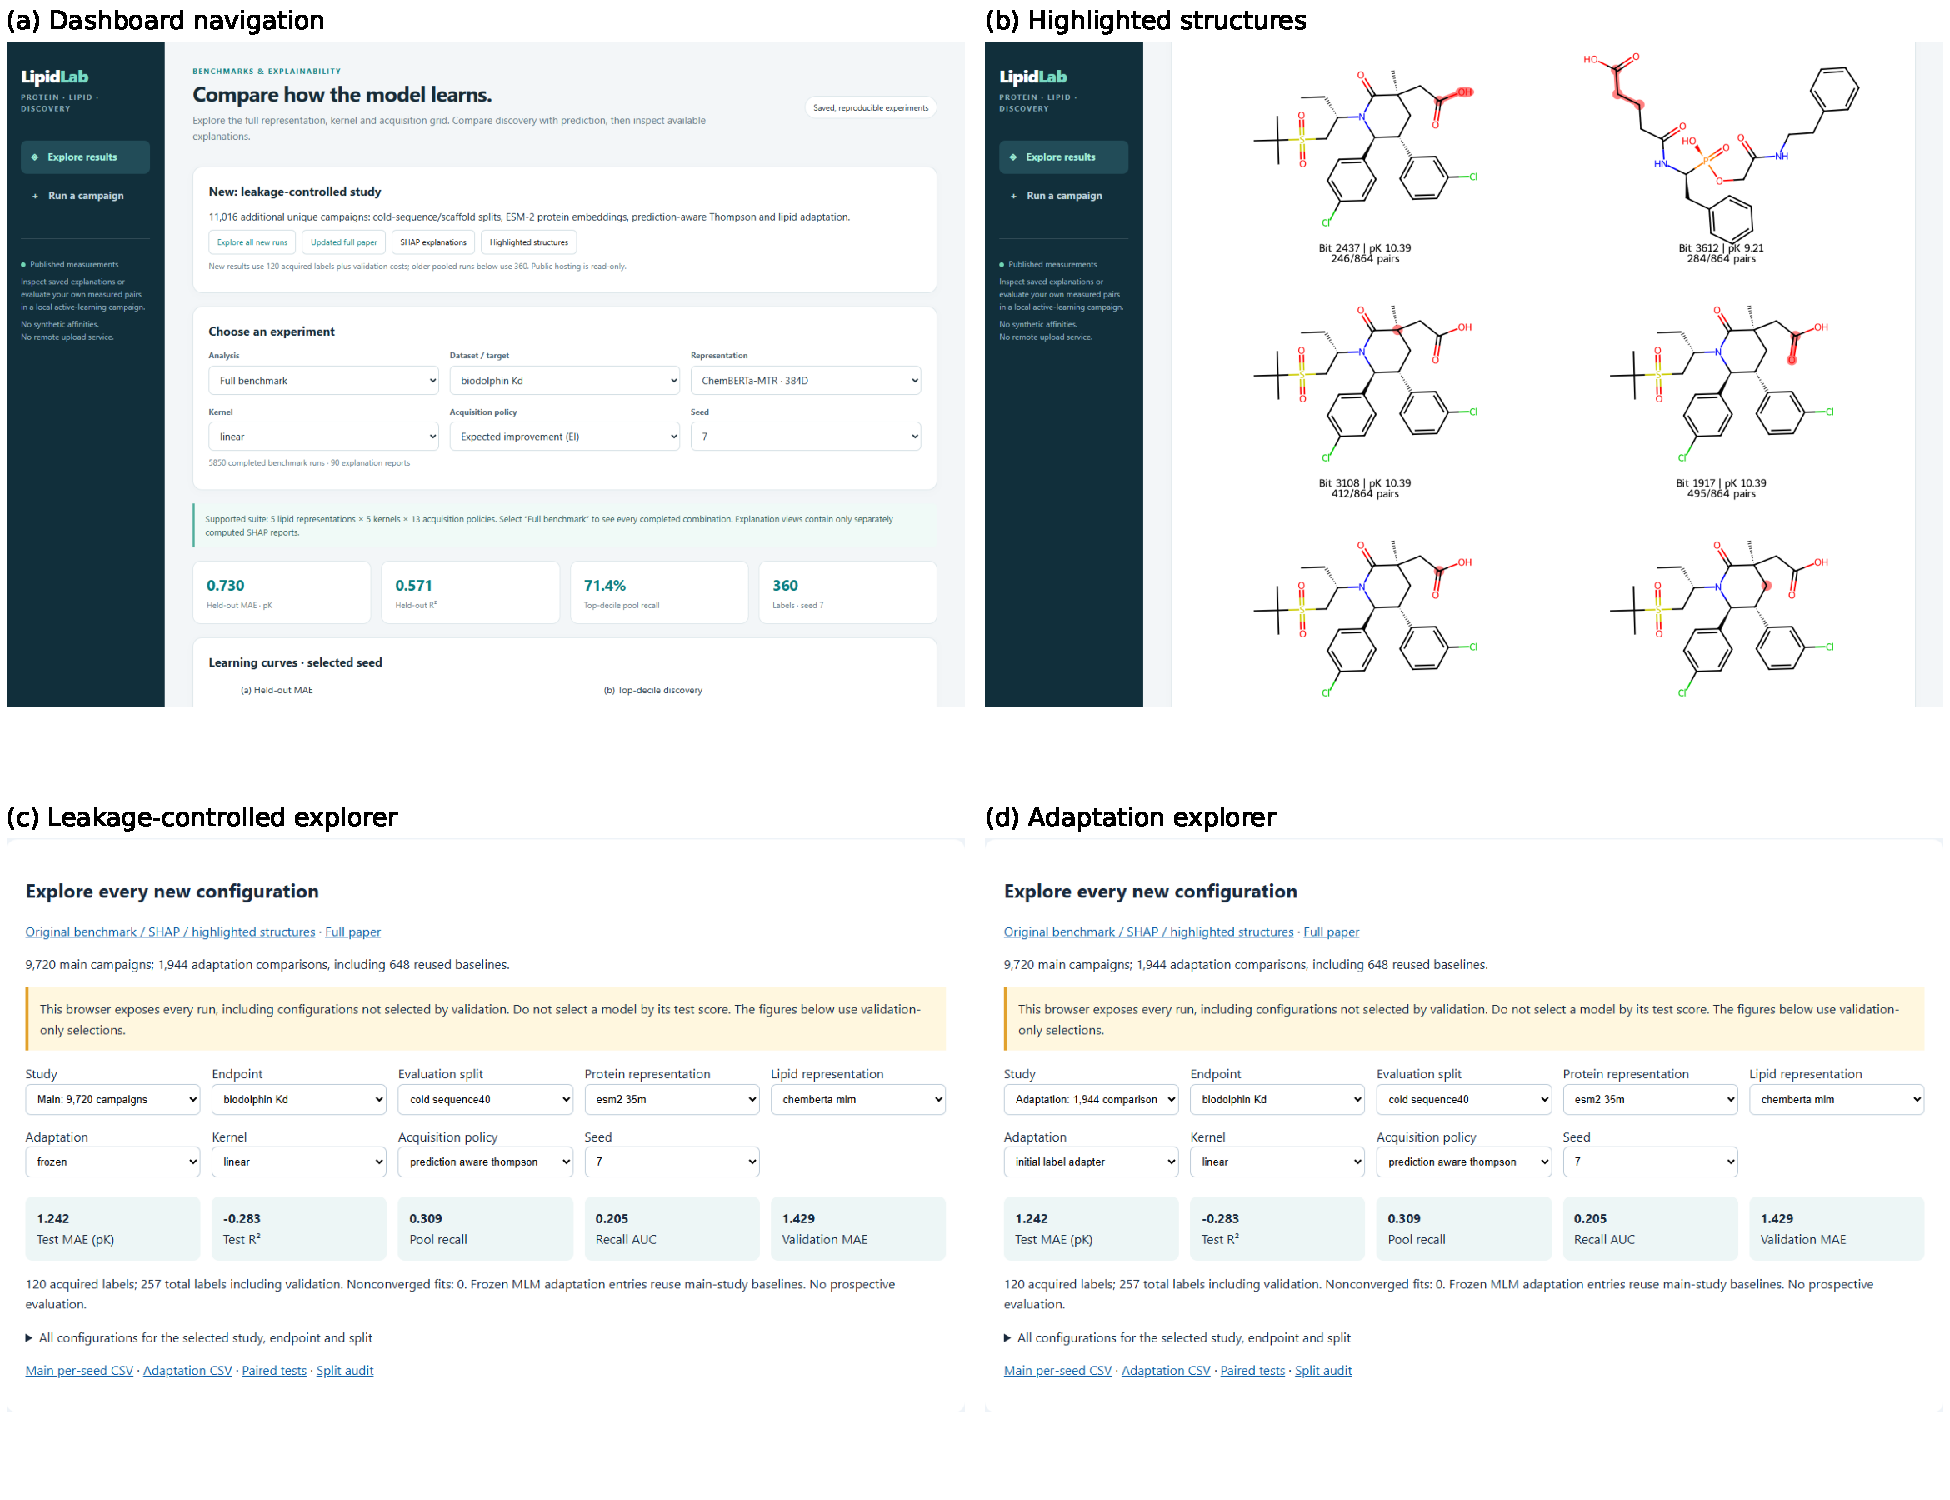
\includegraphics[width=\linewidth]{figures/updated_dashboard.pdf}
\caption{Four genuine screenshots of the updated static dashboard:
original-grid navigation, highlighted fragment view, leakage-controlled
configuration selection, and adaptation selection. Captures use a local
HTTP server serving the generated read-only dashboard, not mockups or evidence of a public
deployment. Hosting status is stated separately in the text.}
\label{fig:dashboard}
\end{figure}

The public export contains allowlisted derived tables, figures, explanations,
and the manuscript. It excludes source datasets, model weights, full GP
checkpoints, private uploaded data, and local environments. Uploading measured
data and running campaigns remain features of the local Python application.
A public AL service would additionally require authenticated uploads,
data-retention rules, persistent job storage, a queue, and bounded workers;
the static site does not claim to provide these.

The original audit records 5,850 campaigns and 48,750 fits, with 26 fits not
meeting the optimizer criterion. The new main audit covers 9,720 campaigns,
48,600 fits, and 23 nonconverged fits. Adaptation checks cover 1,944 comparisons,
36 initial-only adapters, zero benchmark-scaffold overlap in SSL training,
and six nonconverged fits including reused baselines. Initial sets, validation
separation, proxy-label exclusion, selection rules, and data/source hashes
are checked. Convergence flags are retained rather than silently discarded.

Assay heterogeneity remains unresolved. Consensus labels can merge different
conditions; recorded ranges and source annotations are not a full replicate
noise model. Zero observed range does not imply noiseless affinity. Split
control does not remove dataset selection bias, related local domains,
pretraining overlap, or all chemistry similarity. Large cold groups can
change endpoint and chemical distributions. The new work reuses datasets
seen during earlier development, so it is not external validation.

Statistical and biological scope are limited: the tests are underpowered,
the adaptation corpus is small, only one protein-model family is compared,
and contact checks cover selected examples. No prospective measurement or
time-stamped future holdout has been fabricated. Supervised pooled-label
fine-tuning before splitting would leak future labels into AL and is
deliberately not performed. Larger independent corpora, assay-aware modeling,
distinct protein encoder families, and adequately powered prospective studies
remain necessary before stronger claims.

\section{Conclusion}
Protein--lipid AL has distinct predictive and discovery objectives. Explicit
prediction-aware Thompson changes their balance but does not dominate
standard policies. Cold-sequence and scaffold evaluation reveal substantially
harder prediction than random pairs. Frozen protein embeddings and small
lipid adaptation offer mixed gains, while nonlinear/collision/contact
diagnostics make explanations more auditable without making them mechanistic.
The principal outcome is a transparent empirical framework and a qualified
trade-off, not established algorithmic novelty or prospective superiority.

\section*{Supplementary Material}
The source package includes complete per-seed and summary tables for both
evaluation stages, adaptation comparisons, paired tests, split and execution
audits, explanation diagnostics, and hashes. The original atlas retains all
223 historical source figures in four/five-panel composites; an updated
composite supplement includes all seven original main figures, the three new
four-panel comparisons, and the updated dashboard. The main paper uses a
subset to avoid redundant figures. Original data/checkpoints are unchanged.
The adopted ACML template and page budget do not imply current submission
eligibility; author details, anonymity, source redistribution, and scientific
claims require author review before submission.

\begin{thebibliography}{12}
\bibitem[Cohn et~al.(1996)]{cohn1996}
David A. Cohn, Zoubin Ghahramani, and Michael I. Jordan.
Active learning with statistical models. \emph{Journal of Artificial
Intelligence Research}, 4:129--145, 1996.
\doi{10.1613/jair.295}.
\bibitem[DeepChem(n.d.)]{chemberta}
DeepChem. ChemBERTa-77M MTR and MLM checkpoints.
\url{https://huggingface.co/DeepChem/ChemBERTa-77M-MTR};
\url{https://huggingface.co/DeepChem/ChemBERTa-77M-MLM}.
\bibitem[ESM authors(n.d.)]{esm}
ESM authors. ESM-2 pretrained models and implementation.
\url{https://github.com/facebookresearch/esm}.
Pinned checkpoint revisions and pooling details accompany the feature manifest.
\bibitem[Gupta et~al.(2018)]{gupta2018}
Sunil Gupta, Alistair Shilton, Santu Rana, and Svetha Venkatesh.
Exploiting Strategy-Space Diversity for Batch Bayesian Optimization.
Proceedings of AISTATS, PMLR 84:538--547, 2018.
\url{https://proceedings.mlr.press/v84/gupta18a.html}.
\bibitem[Lundberg and Lee(2017)]{lundberg2017}
Scott M. Lundberg and Su-In Lee. A unified approach to interpreting model
predictions. \emph{Advances in Neural Information Processing Systems}, 30, 2017.
\url{https://arxiv.org/abs/1705.07874}.
\bibitem[Rasmussen and Williams(2006)]{rasmussen2006}
Carl Edward Rasmussen and Christopher K. I. Williams.
\emph{Gaussian Processes for Machine Learning}. MIT Press, 2006.
\url{https://gaussianprocess.org/gpml/}.
\bibitem[Rogers and Hahn(2010)]{rogers2010}
David Rogers and Mathew Hahn. Extended-connectivity fingerprints.
\emph{Journal of Chemical Information and Modeling}, 50(5):742--754, 2010.
\doi{10.1021/ci100050t}.
\bibitem[Ross et~al.(2022)]{ross2022}
Jerret Ross, Brian Belgodere, Vijil Chenthamarakshan, Inkit Padhi,
Youssef Mroueh, and Payel Das. Large-scale chemical language representations
capture molecular structure and properties. \emph{Nature Machine Intelligence},
4:1256--1264, 2022. \doi{10.1038/s42256-022-00580-7}.
\bibitem[Russo et~al.(2018)]{russo2018}
Daniel Russo, Benjamin Van Roy, Abbas Kazerouni, Ian Osband, and Zheng Wen.
A tutorial on Thompson sampling. \emph{Foundations and Trends in Machine
Learning}, 11(1):1--96, 2018. \doi{10.1561/2200000070}.
\bibitem[Schrecke et~al.(2021)]{schrecke2021}
Samantha Schrecke, Yun Zhu, Jacob W. McCabe, Mariah Bartz, Charles Packianathan,
Minglei Zhao, Ming Zhou, David Russell, and Arthur Laganowsky.
Selective regulation of human TRAAK channels by biologically active
phospholipids. \emph{Nature Chemical Biology}, 17:89--95, 2021.
\doi{10.1038/s41589-020-00659-5}.
\bibitem[Srivastava et~al.(2026)]{srivastava2026}
Satya Pratik Srivastava, Rohan Gorantla, Sharath Krishna Chundru,
Claire J. R. Winkelman, Antonia S. J. S. Mey, and Rajeev Kumar Singh.
Explainable active learning framework for ligand binding affinity prediction.
\emph{Digital Discovery}, 5:769--779, 2026. \doi{10.1039/D5DD00436E}.
\bibitem[Yang et~al.(2024)]{yang2024}
Li-Yen Yang, Kaike Ping, and Yunan Luo.
BioDolphin as a comprehensive database of lipid--protein binding interactions.
\emph{Communications Chemistry}, 7:288, 2024.
\doi{10.1038/s42004-024-01384-z}.
\end{thebibliography}
\end{document}
